Welcome to the
\href{https://github.com/ENSYSTRA/short-term-forecasting}{short-term-forecasting}
wiki!

Short-term forecasting of electricity generation, demand and prices
using machine learning.

Copyright (C) 2019 Nithiya Streethran.

Permission is granted to copy, distribute and/or modify this document
under the terms of the GNU Free Documentation License, Version 1.3 or
any later version published by the Free Software Foundation; with no
Invariant Sections, no Front-Cover Texts, and no Back-Cover Texts. A
copy of the license is included in the section entitled ``GNU Free
Documentation License''.

Images are licensed under the Creative Commons Attribution-ShareAlike
4.0 International (CC BY-SA 4.0) license, where the image source has not
been specified.

This work is part of Nithiya Streethran's research as Early-Stage
Researcher (ESR) 9 of the \href{https://ensystra.eu/}{ENSYSTRA - ENergy
SYStems in TRAnsition} Innovative Training Network. ENSYSTRA is funded
by the European Union's Horizon 2020 research and innovation programme
under the Marie Skłodowska-Curie grant agreement No: 765515.

\hypertarget{background}{%
\section{Background}\label{background}}

The transition towards a future low-carbon economy is driven globally by
the Paris Agreement \protect\hyperlink{par2015}{{[}par2015{]}}, which
recognises the need for sustainable development worldwide to counter the
threats of climate change. The European Union (EU) is committed to
reduce greenhouse gas (GHG) emissions by 2050 to 80-90 \% below 1990
levels \protect\hyperlink{ene2012}{{[}ene2012{]}}. As the energy
industry is responsible for the highest share of anthropogenic GHG
emissions, importance is placed on how changes in energy systems can
help achieve these GHG emission reduction targets
\protect\hyperlink{ene2012}{{[}ene2012{]}}.

A number of opportunities exist for the decarbonisation of the energy
industry. The International Renewable Energy Agency (IRENA), in their
renewable energy roadmap study, has identified renewable energy as
having the highest potential in reducing energy-related carbon dioxide
(CO2) emissions globally, which is closely followed by energy efficiency
and electrification with renewable energy
\protect\hyperlink{glo0000}{{[}glo0000{]}}. In a 2018 political
agreement, the EU member states agreed upon a target of at least 32 \%
of the demand being met with renewables by 2030, through national
targets of the individual member states
\protect\hyperlink{ren0000}{{[}ren0000{]}}. The electricity demand in
the transport sector is also expected to increase due to expected petrol
and diesel engine bans and subsequently the electrification of road
transport \protect\hyperlink{wor2017}{{[}wor2017{]}}.

According to the EU reference scenario 2016
\protect\hyperlink{ene0000}{{[}ene0000{]}}, wind and solar energy
resources are expected to generate a total of 35 \% of EU's electricity
by 2050. This is a significant increase (23 \%) from 2015 levels.

\begin{longtable}[]{@{}llllllll@{}}
\caption{Characteristics of the main energy generation technologies,
adapted from Erbach 2016 \protect\hyperlink{erb2016}{{[}erb2016{]}} and
Tidball, et al.~2010
\protect\hyperlink{tid2010}{{[}tid2010{]}}.}\tabularnewline
\toprule
Type\protect\hyperlink{f1}{{[}f1{]}} & Variable & Fuel type &
Flexibility & Low carbon & CAPEX\protect\hyperlink{f2}{{[}f2{]}} &
OPEX\protect\hyperlink{f2}{{[}f2{]}} &
LCOE\protect\hyperlink{f2}{{[}f2{]}}\tabularnewline
\midrule
\endfirsthead
\toprule
Type\protect\hyperlink{f1}{{[}f1{]}} & Variable & Fuel type &
Flexibility & Low carbon & CAPEX\protect\hyperlink{f2}{{[}f2{]}} &
OPEX\protect\hyperlink{f2}{{[}f2{]}} &
LCOE\protect\hyperlink{f2}{{[}f2{]}}\tabularnewline
\midrule
\endhead
Coal & no & fossil & medium & no & low & high & very low\tabularnewline
Natural gas & no & fossil & high & no & very low & very high &
low\tabularnewline
Biomass & no & renewable & medium & yes\protect\hyperlink{f3}{{[}f3{]}}
& low & very high & very high\tabularnewline
Nuclear & no & nuclear & low & zero-emission & medium & medium &
medium\tabularnewline
Hydro & no & renewable & very high & zero-emission & & &\tabularnewline
Solar & yes & renewable & very low & zero-emission & very high & very
low & very high\tabularnewline
Wind & yes & renewable & very low & zero-emission & & &\tabularnewline
\emph{Onshore wind} & & & & & high & very low & very low\tabularnewline
\emph{Offshore wind} & & & & & very high & low & high\tabularnewline
Geothermal & no & renewable & high & zero-emission & high & medium &
high\tabularnewline
\bottomrule
\end{longtable}

{[}f1{]} \emph{Costs for natural gas, biomass, solar and geothermal are
that of advanced combustion turbine, biomass gasification plant,
utility-scale photovoltaic and hydrothermal plant respectively}

{[}f2{]} \emph{CAPEX - capital costs; OPEX - operational expenditure
(includes fuel and fixed O\&M costs); LCOE - levelised cost of
electricity}

{[}f3{]} \emph{regrowth of biomass compensates emissions}

\hypertarget{regions}{%
\section{Regions}\label{regions}}

\hypertarget{north-sea-countries}{%
\subsection{North Sea countries}\label{north-sea-countries}}

As per the definition provided by the European MSP Platform
\protect\hyperlink{nor0000}{{[}nor2000{]}} and the CPMR North Sea
Commission \protect\hyperlink{mem2015}{{[}mem2015{]}}, the North Sea
region consists of eight countries: Belgium, Denmark, France, Germany,
Netherlands, Norway, Sweden and United Kingdom.

\hypertarget{nuts-nomenclature-of-territorial-units-for-statistics}{%
\subsubsection{\texorpdfstring{\href{https://ec.europa.eu/eurostat/web/nuts/background}{NUTS
(Nomenclature of territorial units for
statistics)}}{NUTS (Nomenclature of territorial units for statistics)}}\label{nuts-nomenclature-of-territorial-units-for-statistics}}

\href{https://github.com/ENSYSTRA/short-term-forecasting/tree/master/jupyter-notebooks/NUTS.ipynb}{See
the Jupyter notebook}.

\hypertarget{bidding-zones}{%
\subsection{Bidding zones}\label{bidding-zones}}

\hypertarget{definition}{%
\subsubsection{Definition}\label{definition}}

According to \protect\hyperlink{bid2014}{{[}bid2014{]}}:

\begin{itemize}
\tightlist
\item
  The largest geographical area within which market participants are
  able to exchange energy without capacity allocation.
\item
  The majority of bidding zones in Europe are defined by national
  borders (e.g., France or the Netherlands).
\item
  Some are larger than national borders (e.g., Austria, Germany and
  Luxembourg or the Single Electricity Market for the island of Ireland)
\item
  Some are smaller zones within individual countries (e.g., Italy,
  Norway or Sweden).
\end{itemize}

\hypertarget{bidding-zones-in-the-north-sea-region}{%
\subsubsection{Bidding zones in the North Sea
region}\label{bidding-zones-in-the-north-sea-region}}

The bidding zones in the European electricity market are illustrated in
the map below \protect\hyperlink{tre2017}{{[}tre2017{]}}.

\begin{figure}
\centering
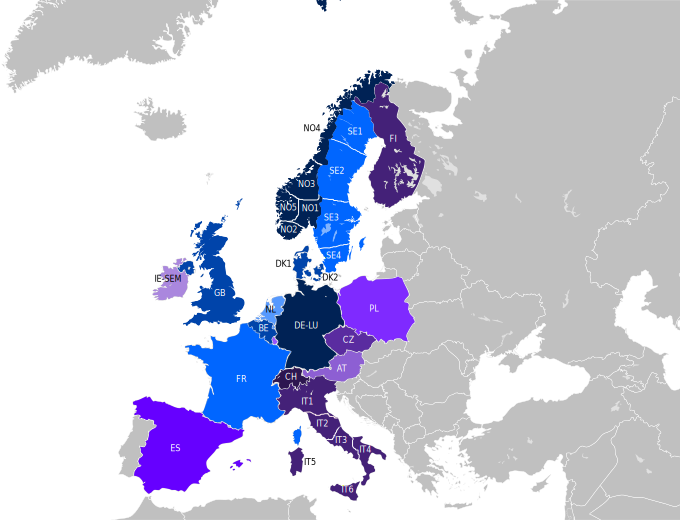
\includegraphics{images/market-map.png}
\caption{Bidding zones in the European electricity market. Source:
\href{http://raport.pse.pl/en/trends-and-market-context}{Polskie Sieci
Elektroenergetyczne}.}
\end{figure}

\begin{longtable}[]{@{}lll@{}}
\caption{Bidding zones in the North Sea region.}\tabularnewline
\toprule
\textbf{Country} & \textbf{Market(s)} & \textbf{Zone(s)}\tabularnewline
\midrule
\endfirsthead
\toprule
\textbf{Country} & \textbf{Market(s)} & \textbf{Zone(s)}\tabularnewline
\midrule
\endhead
Belgium (BE) & EPEX SPOT & BE\tabularnewline
Germany (DE / GE) & EPEX SPOT &
DE-AT-LU\protect\hyperlink{f4}{{[}f4{]}}\tabularnewline
Denmark (DK) & Nord Pool & DK1, DK2\tabularnewline
France (FR) & EPEX SPOT & FR\tabularnewline
Netherlands (NL) & EPEX SPOT & NL\tabularnewline
Norway (NO) & Nord Pool & NO1, NO2, NO3, NO4, NO5\tabularnewline
Sweden (SE / SW) & Nord Pool & SE1, SE2, SE3, SE4\tabularnewline
United Kingdom (UK) & EPEX SPOT, Nord Pool & GB,
I-SEM\protect\hyperlink{f4}{{[}f4{]}}\tabularnewline
\bottomrule
\end{longtable}

{[}f4{]} \emph{Austria (AT / AU); Luxembourg (LU); Great Britain (GB);
Irish single electricity market (I-SEM), which includes Republic of
Ireland (IE) and UK's Northern Ireland (NI)}

\hypertarget{data}{%
\section{Data}\label{data}}

\hypertarget{data-folder-navigation}{%
\subsection{\texorpdfstring{\href{https://drive.google.com/drive/folders/1_3Y30j_c-4iai0WuhcrysXHYdZ4F2AKB}{Data
folder}
navigation}{Data folder navigation}}\label{data-folder-navigation}}

\begin{itemize}
\tightlist
\item
  ENTSO-E

  \begin{itemize}
  \tightlist
  \item
    generation and load data for each bidding zone in the North Sea
    region, grouped by country
  \end{itemize}
\item
  Meteo - meteorological data, grouped by country
\item
  Market - market data for the North Sea region
\item
  NUTS - territorial units
\item
  output - output or modified data from this project
\end{itemize}

\hypertarget{met-data}{%
\subsection{Met data}\label{met-data}}

\hypertarget{deutscher-wetterdienst}{%
\paragraph{\texorpdfstring{\href{https://www.dwd.de/EN/climate_environment/cdc/cdc_node.html}{Deutscher
Wetterdienst}}{Deutscher Wetterdienst}}\label{deutscher-wetterdienst}}

\begin{itemize}
\tightlist
\item
  \href{https://cdc.dwd.de/portal/}{CDC (Climate Data Center) portal}
\item
  \href{https://opendata.dwd.de/climate_environment/CDC/}{CDC OpenData}
\item
  \href{https://opendata.dwd.de/climate_environment/CDC/Terms_of_use.pdf}{Terms
  of use for data on the CDC ftp server}
\item
  Data set descriptions

  \begin{itemize}
  \tightlist
  \item
    \href{https://cdc.dwd.de/sdi/pid/TT_TU_MN009/DESCRIPTION_TT_TU_MN009_en.pdf}{Hourly
    station observations of air temperature at 2 m above ground in °C
    for Germany}
  \item
    \href{https://cdc.dwd.de/sdi/pid/RF_TU_MN009/DESCRIPTION_RF_TU_MN009_en.pdf}{Hourly
    station observations of relative humidity in \% for Germany}
  \item
    \href{https://cdc.dwd.de/sdi/pid/R1_MN008/DESCRIPTION_R1_MN008_en.pdf}{Hourly
    station observations of precipitation amount in mm for Germany}
  \item
    \href{https://cdc.dwd.de/sdi/pid/WRTR_MN008/DESCRIPTION_WRTR_MN008_en.pdf}{Hourly
    station observations of form of precipitation (WR code) for Germany}
  \item
    \href{https://cdc.dwd.de/sdi/pid/RS_IND_MN008/DESCRIPTION_RS_IND_MN008_en.pdf}{Hourly
    station observations of index whether precipitation has fallen for
    Germany}
  \item
    \href{https://cdc.dwd.de/sdi/pid/F_MN003/DESCRIPTION_F_MN003_en.pdf}{Hourly
    mean of station observations of wind speed ca. 10 m above ground in
    m/s for Germany}
  \item
    \href{https://cdc.dwd.de/sdi/pid/D_MN003/DESCRIPTION_D_MN003_en.pdf}{Hourly
    mean of station observations of wind direction at ca. 10 m above
    ground in degree for Germany}
  \item
    \href{https://cdc.dwd.de/sdi/pid/P0_MN008/DESCRIPTION_P0_MN008_en.pdf}{Hourly
    station observations of air pressure at station level in hpa for
    Germany}
  \item
    \href{https://cdc.dwd.de/sdi/pid/P_MN008/DESCRIPTION_P_MN008_en.pdf}{Hourly
    station observations of air pressure at mean sea level in hpa for
    Germany}
  \item
    \href{https://cdc.dwd.de/sdi/pid/N_MN008/DESCRIPTION_N_MN008_en.pdf}{Hourly
    station observations of cloud coverage in eighths for Germany}
  \end{itemize}
\item
  \href{https://opendata.dwd.de/climate_environment/CDC/observations_germany/climate/hourly/wind/}{Hourly
  wind data}
\end{itemize}

\hypertarget{royal-netherlands-meteorological-institute}{%
\paragraph{\texorpdfstring{\href{https://data.knmi.nl/datasets}{Royal
Netherlands Meteorological
Institute}}{Royal Netherlands Meteorological Institute}}\label{royal-netherlands-meteorological-institute}}

\hypertarget{met-office}{%
\paragraph{\texorpdfstring{\href{https://www.metoffice.gov.uk/datapoint}{Met
Office}}{Met Office}}\label{met-office}}

\hypertarget{norwegian-meteorological-institute}{%
\paragraph{\texorpdfstring{\href{https://www.met.no/en/free-meteorological-data}{Norwegian
Meteorological
Institute}}{Norwegian Meteorological Institute}}\label{norwegian-meteorological-institute}}

\hypertarget{swedish-meteorological-and-hydrological-institute}{%
\paragraph{\texorpdfstring{\href{https://www.smhi.se/en/services/professional-services/data-and-statistics}{Swedish
Meteorological and Hydrological
Institute}}{Swedish Meteorological and Hydrological Institute}}\label{swedish-meteorological-and-hydrological-institute}}

\hypertarget{danish-meteorological-institute}{%
\paragraph{\texorpdfstring{\href{http://research.dmi.dk/data/}{Danish
Meteorological
Institute}}{Danish Meteorological Institute}}\label{danish-meteorological-institute}}

\hypertarget{muxe9tuxe9o-france}{%
\paragraph{\texorpdfstring{\href{https://donneespubliques.meteofrance.fr/}{Météo-France}}{Météo-France}}\label{muxe9tuxe9o-france}}

\hypertarget{the-royal-meteorological-institute-of-belgium}{%
\paragraph{\texorpdfstring{\href{https://opendata.meteo.be/}{The Royal
Meteorological Institute of
Belgium}}{The Royal Meteorological Institute of Belgium}}\label{the-royal-meteorological-institute-of-belgium}}

\hypertarget{generation-and-demand-data}{%
\subsection{Generation and demand
data}\label{generation-and-demand-data}}

\hypertarget{entso-e-transparency-platform}{%
\paragraph{\texorpdfstring{\href{https://transparency.entsoe.eu/}{ENTSO-E
Transparency
Platform}}{ENTSO-E Transparency Platform}}\label{entso-e-transparency-platform}}

\begin{itemize}
\tightlist
\item
  \href{https://docstore.entsoe.eu/Documents/MC\%20documents/Transparency\%20Platform/ENTSOE_Transparency_Terms_Conditions.pdf}{GENERAL
  TERMS AND CONDITIONS FOR THE USE OF THE ENTSO-E TRANSPARENCY PLATFORM}
\item
  \href{https://docstore.entsoe.eu/Documents/MC\%20documents/Transparency\%20Platform/List_of_Data_available_for_reuse.pdf}{LIST
  OF DATA AVAILABLE FOR FREE RE-USE}
\item
  Downloaded data:

  \begin{itemize}
  \tightlist
  \item
    \href{https://transparency.entsoe.eu/generation/r2/actualGenerationPerProductionType/show}{Actual
    Generation per Production Type}
  \item
    \href{https://transparency.entsoe.eu/load-domain/r2/totalLoadR2/show}{Total
    Load - Day Ahead / Actual}
  \end{itemize}
\end{itemize}

\hypertarget{market-data}{%
\subsection{Market data}\label{market-data}}

\hypertarget{nord-pool}{%
\paragraph{\texorpdfstring{\href{https://www.nordpoolgroup.com/historical-market-data/}{Nord
Pool}}{Nord Pool}}\label{nord-pool}}

\begin{itemize}
\tightlist
\item
  \href{https://www.nordpoolgroup.com/trading/join-our-markets/membership/}{Membership
  list - Nord Pool}
\item
  \href{https://www.nordpoolgroup.com/About-us/Terms-and-conditions-for-use/}{Terms
  and conditions for use}
\end{itemize}

\hypertarget{epex-spot}{%
\paragraph{\texorpdfstring{\href{https://www.epexspot.com/en/extras/download-center/market_data}{EPEX
Spot}}{EPEX Spot}}\label{epex-spot}}

\begin{itemize}
\tightlist
\item
  \href{https://www.epexspot.com/en/membership/list_of_members}{EPEX
  SPOT Exchange Members}
\end{itemize}

\hypertarget{other-data}{%
\subsection{Other data}\label{other-data}}

\hypertarget{nuts-nomenclature-of-territorial-units-for-statistics-1}{%
\paragraph{\texorpdfstring{\href{https://ec.europa.eu/eurostat/web/gisco/geodata/reference-data/administrative-units-statistical-units/nuts}{NUTS
(Nomenclature of territorial units for
statistics)}}{NUTS (Nomenclature of territorial units for statistics)}}\label{nuts-nomenclature-of-territorial-units-for-statistics-1}}

\hypertarget{methodology}{%
\section{Methodology}\label{methodology}}

\hypertarget{modelling-framework}{%
\subsection{Modelling framework}\label{modelling-framework}}

\begin{figure}
\centering
\includegraphics{images/model_framework.jpg}
\caption{Modelling framework.}
\end{figure}

\hypertarget{references}{%
\section{References}\label{references}}

{[}bid2014{]} `Bidding Zones Literature Review'. Ofgem, July 2014.
\url{https://www.ofgem.gov.uk/sites/default/files/docs/2014/10/fta_bidding_zone_configuration_literature_review_1.pdf}.

{[}ene0000{]} `Energy Modelling - EU Reference Scenario 2016'. Accessed
1 November 2018.
\url{https://data.europa.eu/euodp/data/dataset/energy-modelling}.

{[}ene2012{]} Energy roadmap 2050, 2012. Publications Office of the
European Union, Luxembourg. \url{https://doi.org/10.2833/10759}.

{[}erb2016{]} Erbach, Gregor. `Understanding Electricity Markets in the
EU'. Briefing. European Union, November 2016.
\url{http://www.europarl.europa.eu/RegData/etudes/BRIE/2016/593519/EPRS_BRI(2016)593519_EN.pdf}.

{[}glo0000{]} `Global Energy Transformation: A Roadmap to 2050'.
International Renewable Energy Agency. Accessed 14 November 2018.
\url{http://www.irena.org/publications/2018/Apr/Global-Energy-Transition-A-Roadmap-to-2050}.

{[}mem2015{]} `Member Directory \textbar{} Map -- CPMR North Sea
Commission', 21 October 2015.
\url{https://cpmr-northsea.org/who-we-are/member-directory-map/}.

{[}nor0000{]} `North Sea \textbar{} European MSP Platform'. Accessed 1
June 2018. \url{https://www.msp-platform.eu/sea-basins/north-sea-0}.

{[}par2015{]} `Paris Agreement'. United Nations Framework Convention on
Climate Change, 2015.
\url{https://unfccc.int/process-and-meetings/the-paris-agreement/the-paris-agreement}.

{[}ren0000{]} `Renewable Energy - Energy - European Commission'. Energy.
Accessed 12 October 2018.
\url{https://ec.europa.eu/energy/en/topics/renewable-energy}.

{[}tid2010{]} Tidball, R, J Bluestein, N Rodriguez, S Knoke, ICF
International, and J Macknick. `Cost and Performance Assumptions for
Modeling Electricity Generation Technologies'. Subcontract Report.
National Renewable Energy Laboratory, 2010.
\url{https://www.nrel.gov/docs/fy11osti/48595.pdf}.

{[}tre2017{]} `Trends and Market Context'. PSE Impact Report. PSE, 2017.
\url{http://raport.pse.pl/en/trends-and-market-context}.

{[}wor2017{]} `World Energy Outlook 2017'. Paris, France: International
Energy Agency, 2017. \url{https://www.iea.org/weo2017/}.
